
% Титульный слайд
\begin{frame}[noframenumbering, plain]
    \setcounter{framenumber}{1}
    \maketitle
\end{frame}

\section{Введение}

\begin{frame}{Постановка задачи}
	\textbf{\underline{Цель диссертационной работы}}: разработка методики коррекции расчетных моделей летательных аппаратов по результатам модальных испытаний.
	\begin{center}
		\includegraphics[width = 0.6\textwidth]{large-reflector}
	\end{center}
\end{frame}

\begin{frame}{Алгоритм решения проблемы}
	\begin{columns}
		\begin{column}{0.5\textwidth}
			\centering
			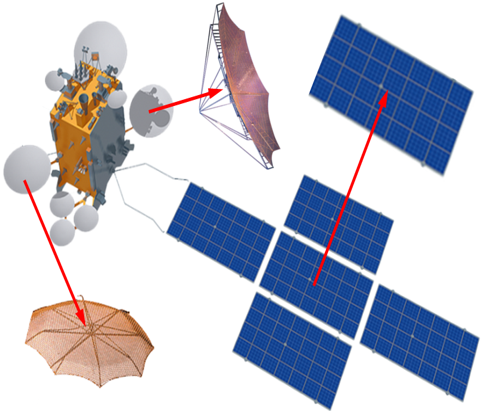
\includegraphics[width=1\textwidth]{decomposition}
		\end{column}
		\begin{column}{0.5\textwidth}
			\centering
			% Определение стиля
			\tikzstyle{blockWide}=[rectangle, draw = black, fill = blue!20, rounded corners, text width = 20em, text centered, minimum height = 1.5em, drop shadow] % Блок
			\tikzstyle{blockWideC}=[blockWide, fill = red!20]
			\tikzstyle{arrow} = [draw, thick, color=black!90, -latex'] % Стрелка
			\scriptsize % Размер шрифта
			% Задание перменных
			\def\nodeDist{0.3cm} % Дистанция между узлами
			% Отрисовка блок-схемы
			\begin{tikzpicture}[scale = 1, transform shape]
				% Задание узлов		
				\node (modalTests) [blockWide] {Модальные испытания составных частей конструкции};
				\node (modelUpdating) [blockWide, below = \nodeDist of modalTests] {Коррекция расчетных моделей составных частей конструкции по результатам испытаний};
				\node (checkInfluence) [blockWide, below = \nodeDist of modelUpdating] {Освобождение закрепленных расчетных моделей составных частей конструкции};
				\node (buildRealModel) [blockWide, below = \nodeDist of checkInfluence] {Синтез расчетной модели полной конструкции из её составных частей};
				\node (buildMathModel) [blockWide, below = \nodeDist of buildRealModel] {Определение динамических характеристик полной расчетной модели};
				% Соединение узлов
				\draw [arrow] (modalTests.south) -- (modelUpdating.north);
				\draw [arrow] (modelUpdating.south) -- (checkInfluence.north);
				\draw [arrow] (checkInfluence.south) -- (buildRealModel.north);
				\draw [arrow] (buildRealModel.south) -- (buildMathModel.north);
			\end{tikzpicture}
		\end{column}
	\end{columns}
\end{frame}

\begin{frame}{Задачи исследования}
	\begin{enumerate}
		\item Разработать методику коррекции расчетных динамических моделей ЛА по экспериментально определенным модальным характеристикам.
		\item Изучить методы классического модального анализа. Создать комплекс программ для обработки и представления результатов модального анализа непосредственно в процессе испытаний.
		\item Изучить методы операционного модального анализа. Разработать программное обеспечение для определения модальных характеристик ЛА по результатам акустических и летных испытаний.
		\item Изучить методы вибродиагностики конструкций. Разработать программное обеспечение для контроля конструктивно-производственных дефектов в конструкциях ЛА в процессе модальных испытаний.
		\item Оценить сходимость и чувствительность методики коррекции к погрешностям в результатах модальных испытаний.
		\item Решить практические задачи коррекции расчетных моделей конструкций.
	\end{enumerate}
\end{frame}

\begin{frame}{Положения, выносимые на защиту}
	\begin{enumerate}
		\item Методика коррекции расчетных динамических моделей путем добавления корректирующих конечных элементов, параметры которых определяются из решения задачи оптимизации по целевым модальным характеристикам.
		\item Методика синтеза расчетной модели ЛА из полноразмерных моделей составных частей, скорректированных по результатам модальных испытаний.
		\item Комплекс программ для обработки и представления результатов экспериментального модального анализа. Программное обеспечение коррекции и синтеза расчетных моделей ЛА.
		\item Результаты исследования сходимости алгоритма и чувствительности методики коррекции расчетных моделей к погрешностям эксперимента.
		\item Результаты решения практических задач.
	\end{enumerate}
\end{frame}

\begin{frame}{Обзор публикаций по теме исследования}
	\begin{itemize}
		\item \textbf{Стохастические методы коррекции}: \\ Beck~J.\,L., Katafygiotis~L.\,S., Boulkaibet~I., Vanik~M.\,W., Goller~B., Schueller~G.\,I., Au~S.\,K., Marwala~T., Yuen~K.\,V., Worden~K., Hensman~J.\,J., Cheung~S.\,H., Mthembu~L., Yan~W.\,J.
		\item \textbf{Детерминированные методы коррекции}: \\ Bakir~P.\,G., Friswell~M.\,I., Baruch~M., Mottershead~J.\,E., Ewins~D.\,J., Berman~E.\,G., Allen~M.\,S., Link~M., Park~D.\,C., Caesar~B., Min~C.\,H., Sipple~J.\,D., Gupta~A.
		\item \textbf{Методы регуляризации}: \\ Ahmadian~H., Fregolent~A., Natke~H.\,G., Visser~W.\,J., Titurus~B., Imregun~M., D'Ambrogio~W., Gladwell~G.\,M.\,L., Ismail~F., Hansen~P.\,C., Bartilson~D.\,T., Smyth~A.\,W.
		\item \textbf{Теоретические и практические аспекты методов модальных испытаний}: \\ Резник~А.\,Л., Смыслов~В.\,И., Микишев~Г.\,Н., Рабинович~Б.\,И., Бернс~В.\,А., Dat~R., Clerc~D., Kennedy~C.\,C., Pancu~C.\,D.\,P., Heylen~W., Lammens~S., Sas~P.
	\end{itemize}
\end{frame}